\chapter{Marshaling between C\# and C}
For this chapter, you'll need to create a ChapterFive directory and initialize a Dotnet Console project and to reference ''AdvancedDLSupport'' from nuget.

\section{Struct Layout}
The Layout in Struct is by default set to Sequential and you cannot use Auto layout for marshaling between Managed and Unmanaged code. Explicit Layout allows the you to explicitly define the field offsets in struct layout. This is also what enables you to  create a union in struct.

\lstinputlisting[style=customcs]{codes/Chap5/Chap5Snippet1.cs}

You may have noticed that the Val1 occupied 2 byte slots in the struct rather than Val2 being placed immediately after Val1. This is due to data alignment.  More information on that can be found here: https://software.intel.com/en-us/articles/data-alignment-when-migrating-to-64-bit-intel-architecture

To quote from that link:

\begin{coloredbox}
	The fundamental rule of data alignment is that the safest (and most widely supported) approach relies on what Intel terms "the natural boundaries." Those are the ones that occur when you round up the size of a data item to the next largest size of two, four, eight or 16 bytes. For example, a 10-byte float should be aligned on a 16-byte address, whereas 64-bit integers should be aligned to an eight-byte address. Because this is a 64-bit architecture, pointer sizes are all eight bytes wide, and so they too should align on eight-byte boundaries. - Intel 2018
\end{coloredbox}

The size of the struct shown above is 12 bytes rather than 8 bytes, because the sequential layout rule was being followed. However if you wish to override the behavior on data alignment, you can use Explicit Layout as shown below:
\newpage
\lstinputlisting[style=customcs]{codes/Chap5/Chap5Snippet2.cs}

In this struct, the size would become 8 bytes, because there is no padding required for any dangling member to fits in alignment, so everything fits neatly inside the 8 bytes boundary. Also, in explicit layout, the arrangement of members in struct does not affect how memory is laid out, you define the offsets yourself, so you essentially can arrange the members however you like, though it's recommended to keep member arrangement sequential for readability.

\subsection{Union}
Due to the nature of explicit layout, we can overlap where the field are located in memory by using FieldOffset. If you have for an example have the following code:

\lstinputlisting[style=customcs]{codes/Chap5/Chap5Snippet3.cs}

The size of struct would remain at 1 byte, so no padding is added and both fields are storing into the same memory in the struct.

It is however recommended that you create separate structs for each union definition that you may come across in C native library binding as demonstrated:

\lstinputlisting[style=customcs]{codes/Chap5/Chap5Snippet4.cs}

The resulting size of this struct would be 8 bytes, because it still follows the padding rule for sequential in MyStruct by padding the union struct to fits in the memory boundary.

\subsection{Packing and Size Options for Struct Layout}
You can specify the packing option to respect byte boundary from a multiple of 1 byte to 8 bytes (.Net Core 3.0 and later will support 16 to 32 bytes boundary.)

Size will only be respected if the specified size is bigger than actual size of struct (including padding).

Here an example to demonstrate the differences of each struct with specified Packing and Size.

\lstinputlisting[style=customcs]{codes/Chap5/Chap5Snippet5.cs}
\newpage
And the output for each struct is as followed:
\newline \newline
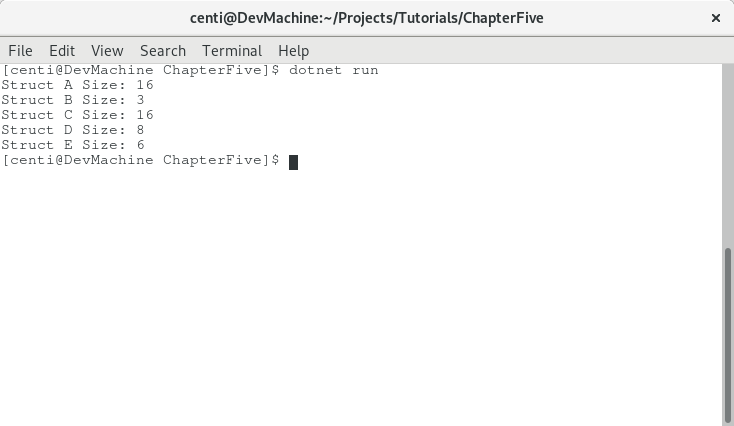
\includegraphics[width=\textwidth]{ChapFiveConsole}

\begin{enumerate}
	\item Struct A have Size specified and is larger than the actual size of struct with padding (which is 1 byte size for Struct A actual size.)
	\item Struct B have Size specified to be smaller than the actual size of Struct, therefore the size parameter is ignored for this layout, the size for this struct become 3 bytes. It also isn't padded to the multiple of 4 or 8, because 3 bytes can be aligned in a single 4 bytes word as described by intel's Natural Boundaries.
	\item Struct C size is 16 bytes even though it's actual size is 9 bytes, this is how padding affects the size of the struct. If padding is set to 1, we would see the Struct C size become 9 bytes long.
	\item Struct D size is 8 bytes as described above, the actual size of struct is 5 bytes long and because of the specified padding, it is padded to 8 bytes boundary.
	\item Struct E size is 6 bytes as opposed to Struct D, because packing is specified to pad struct to the multiple of 2 bytes.
\end{enumerate}

\subsection{Technical Note on Packing}
While Natural Boundaries are something to keep in mind for 64 bit data alignment, it is done differently for 32 bit architecture, it's packed in the multiple of 4 bytes. And in CoreCLR prior to 3.0, 8 bytes packing is the most that can be used and .Net Core 3.0 and later will have packing supporting 16 and 32 bytes boundary to support Vector128<T> and Vector256<T>. 

\subsection{What is the Difference between sizeof and Marshal.SizeOf}
Marshal.SizeOf tells you how much bytes are needed to allocate the structure in unmanaged environment and sizeof tells you how much memory required to allocate the structure in managed environment. The SIzeOf keyword cannot accept managed object, but Unsafe.SizeOf can and it utilize the underlying CIL sizeof opcode.

Let's assume we have the following code to demonstrate the difference:

\lstinputlisting[style=customcs]{codes/Chap5/Chap5Snippet6.cs}

And the output of that program will be:
\newline
\newline
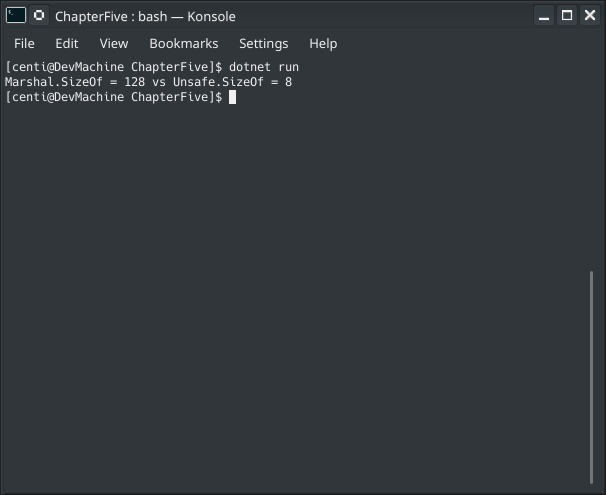
\includegraphics[width=\textwidth]{ChapFiveConsoleTwo}
\newpage

In a managed environment, the string would be a reference type and on 64 bit architecture, the pointer would be 8 bytes long, 4 bytes long on a 32 bit architecture. However, because we explicitly define that our string in a struct is a By Value String, it is essentially a fixed length array of characters of specific encoding (in this case, Ansi Encoding.) The size of struct \textit{should} be 128 bytes long for marshaling purpose.
\subsection{Fixed Size Array}

\subsection{Array of Struct}

\section{Pointer Marshaling}

\section{Function Marshaling}

